\documentclass[12pt,a4paper,oneside]{article}
\usepackage[colorlinks=true, unicode]{hyperref}
\usepackage[utf8]{inputenc}
\usepackage[czech]{babel}
\usepackage{graphicx}
\usepackage{pdfpages}
\textwidth 16cm \textheight 25cm
\topmargin -1.3cm 
\oddsidemargin 0cm
\usepackage{footnote}
\pagestyle{empty}
\begin{document}
\title{Linkový RF zesilovač - GB01A}
\author{Jakub Kákona, kaklik@mlab.cz}
\maketitle

\thispagestyle{empty}
\begin{abstract}
Modul určený k zesílení RF signálu například na vstupu přijímače.
Poskytuje širokopásmový zisk zvolený podle osazeného MMIC obvodu.
\end{abstract}

\begin{figure} [htbp]
\begin{center}
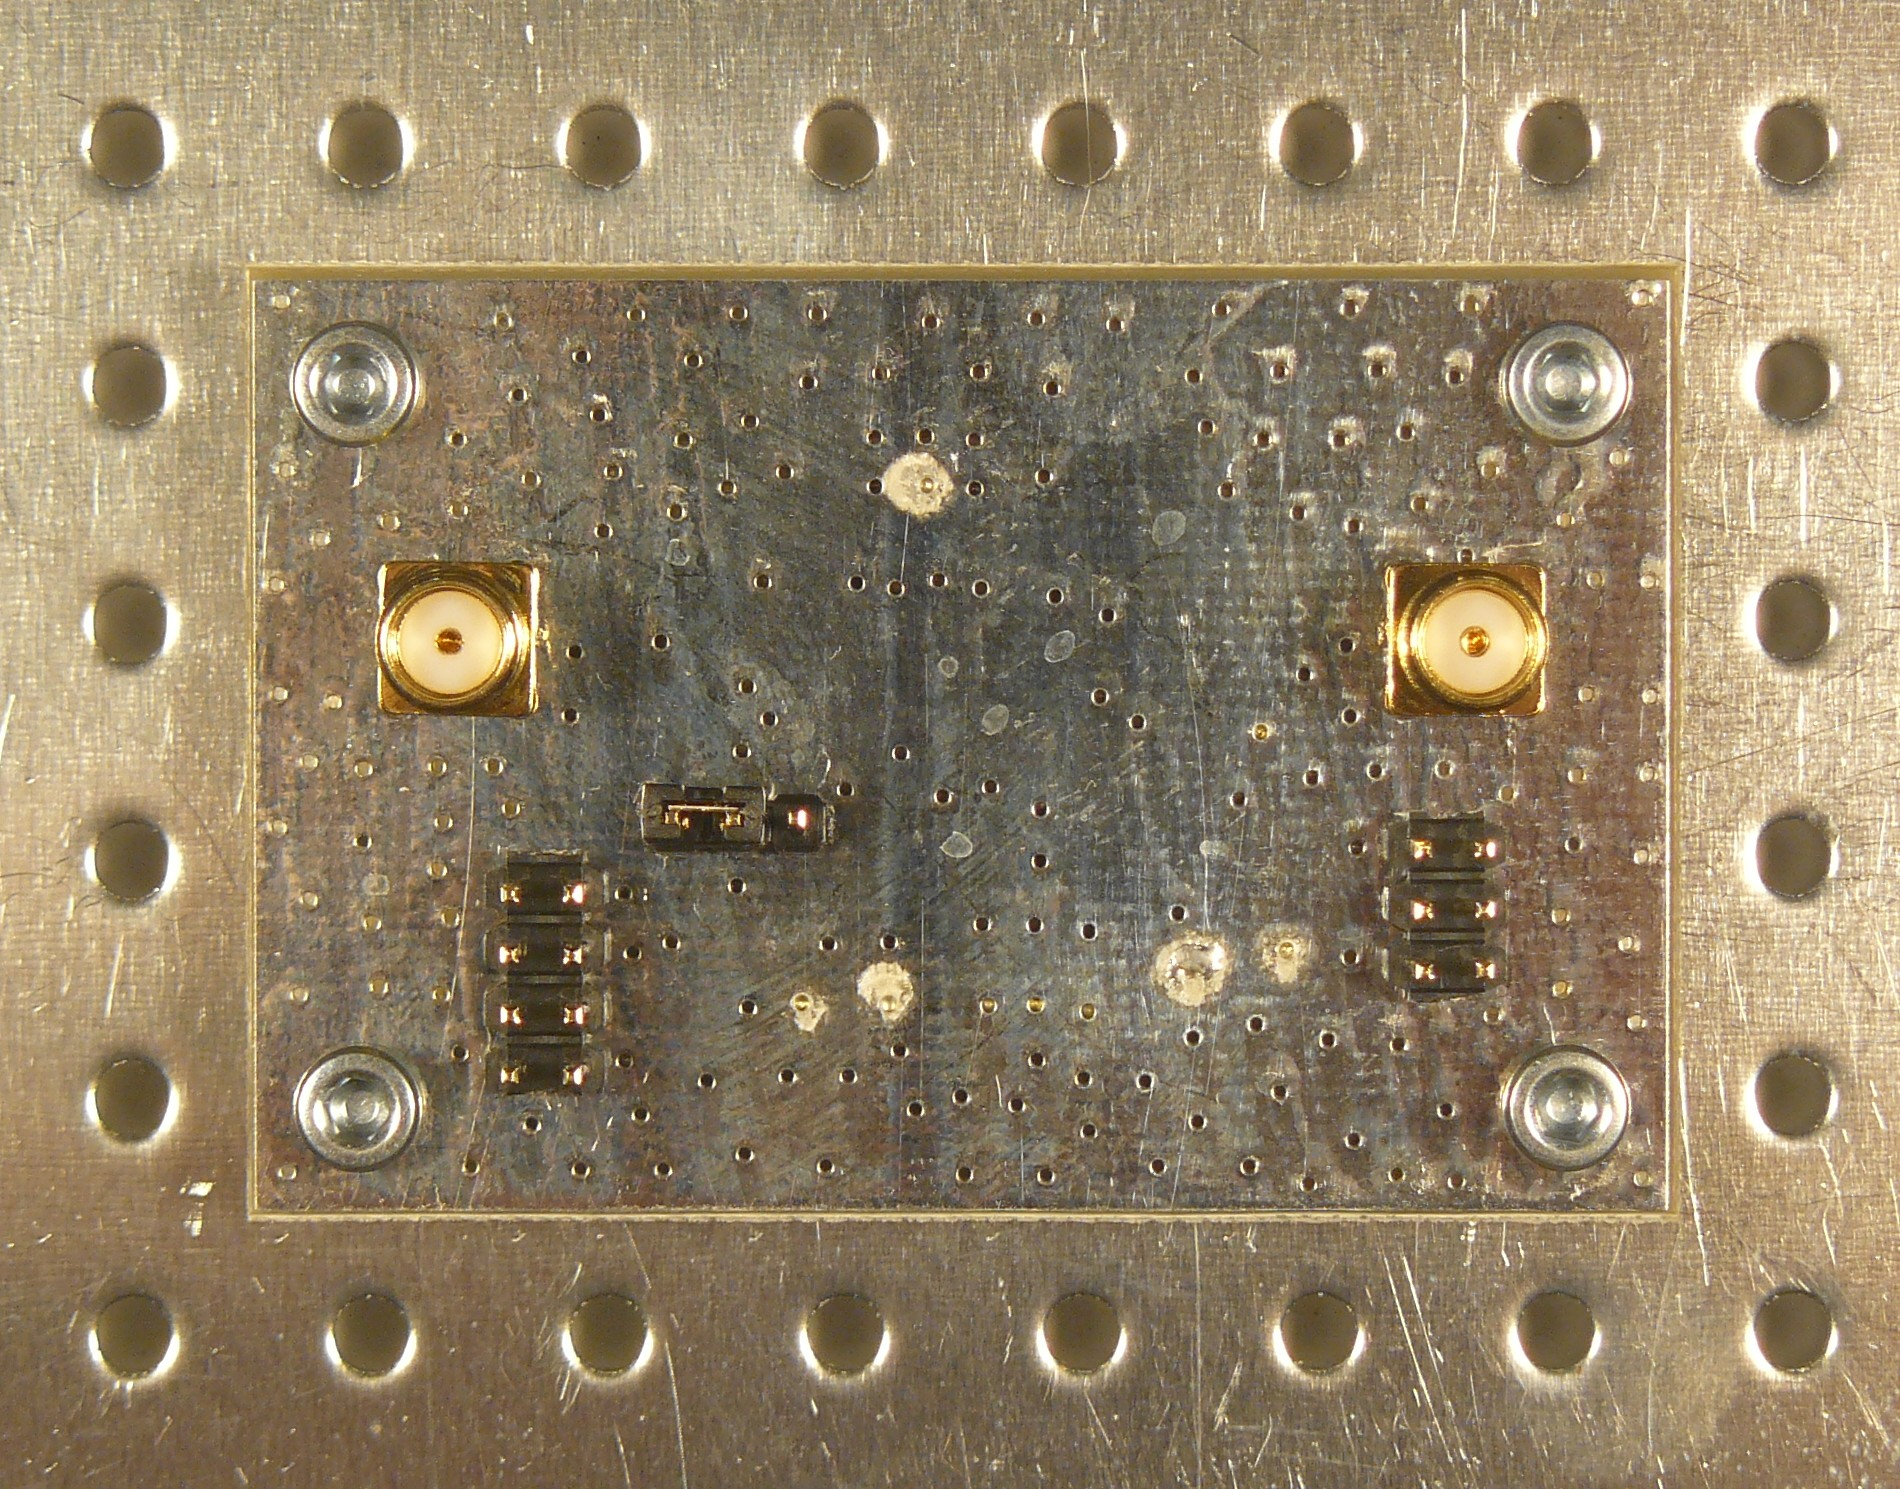
\includegraphics [width=80mm] {./img/GB01A_Top_Big.JPG} 
\end{center}
\end{figure}

\begin{figure} [b]

\includegraphics [width=25mm] {./img/GB01A_QRcode.png} 
\end{figure}

\newpage
\tableofcontents

\section{Technické parametry}
\begin{table}[htbp]
\begin{center}
\begin{tabular}{|c|c|p{4.7cm}|}
\hline
Parametr & Hodnota & Poznámka \\
\hline
Napájecí napětí  & max 12V &  130mA \\ 
\hline
Frekvenční rozsah  & 20 - 1000 MHz & Záleží na konkrétním typu osazeného obvodu \\ 
\hline
\end{tabular}
\end{center}
\end{table}

\section{Popis konstrukce}

Modul linkového zesilovače je konstruován pro univerzální širokopásmové zesílení. Může být také využit jako napájecí výhybka. 

\subsection{Zapojení}

Zapojení je navrženo tak, aby zesilovač mohl být napájen po výstupním koaxiálním kabelu a aby toto napájení mohlo být sdíleno s dalšími komponentami zapojenými před zesilovač. Typicky jde například o LNA. Jestli tato možnost bude využita závisí na konfiguraci jumperu. 

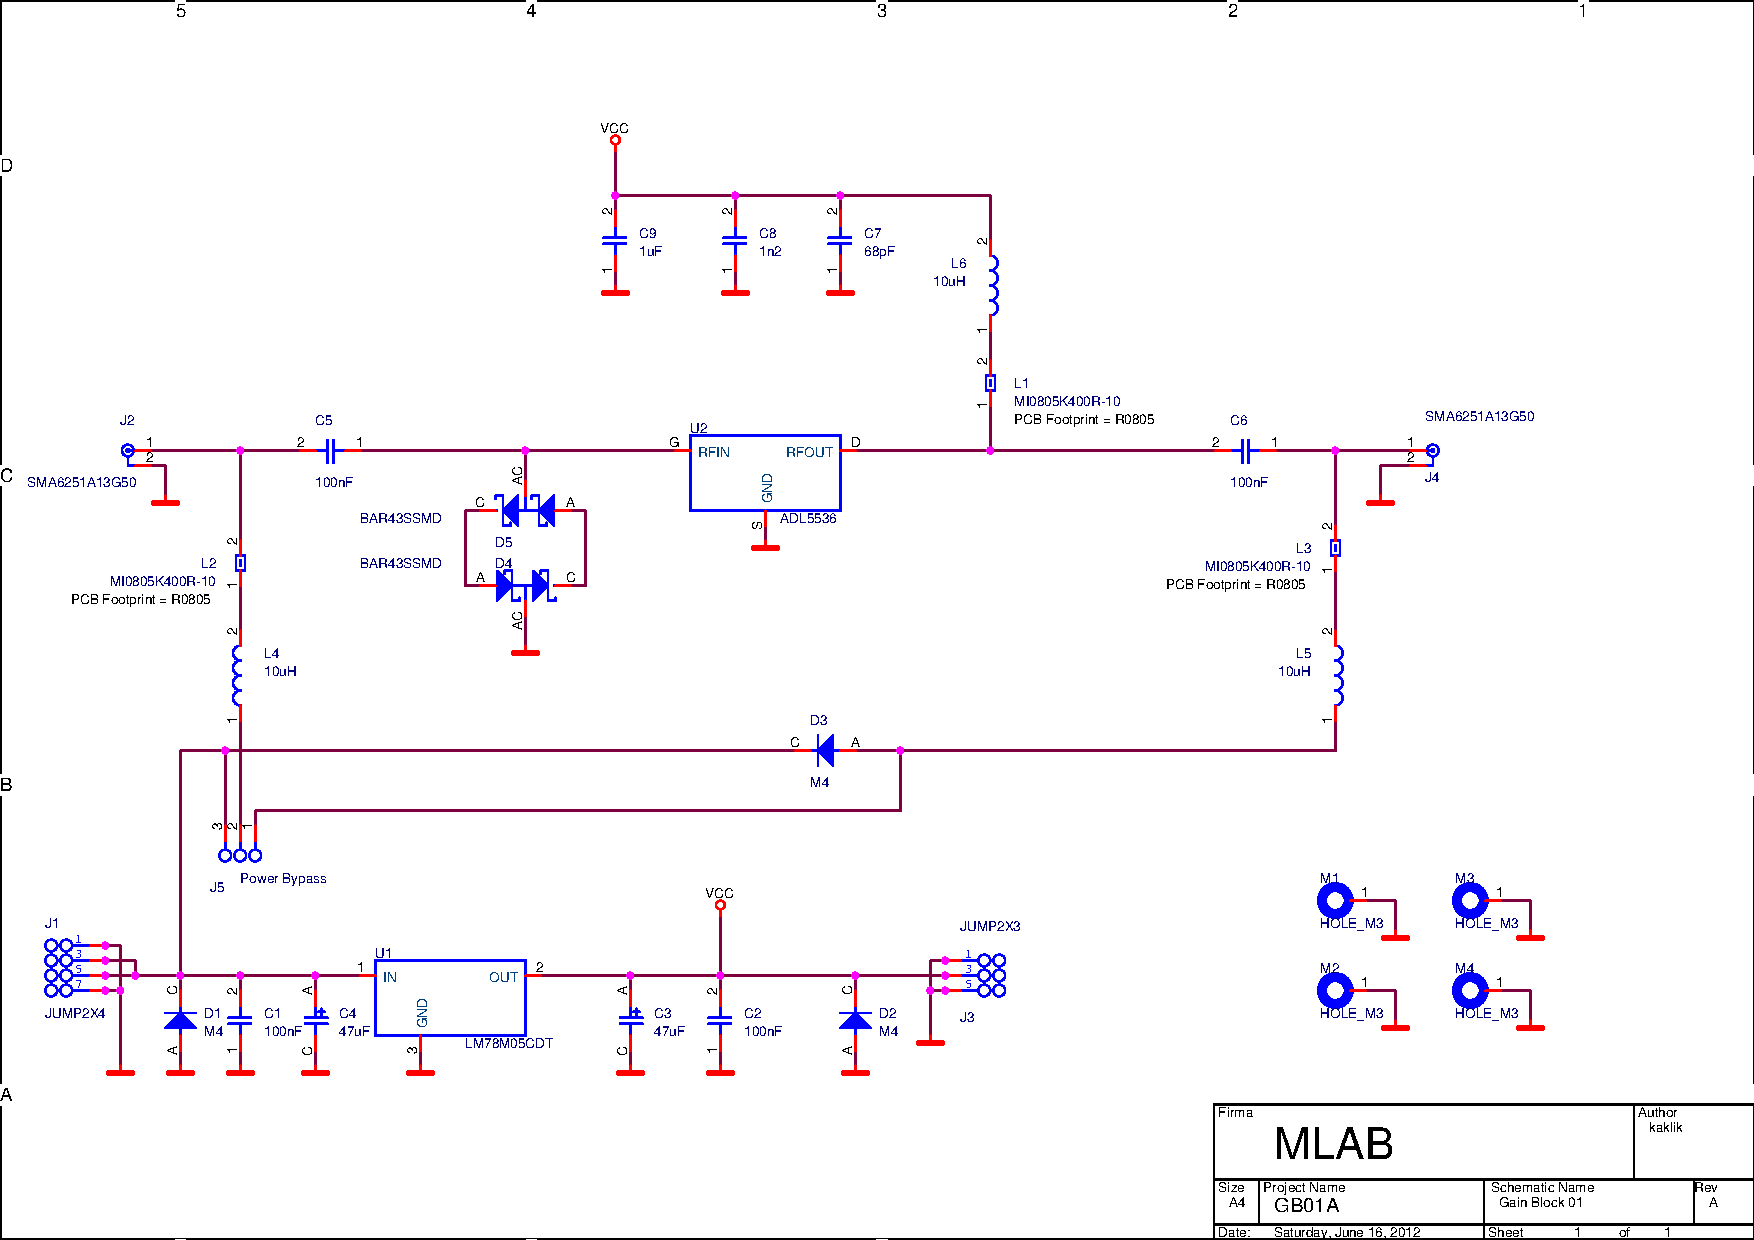
\includepdf[pages={1},landscape=true]{../../SCH/GB01A.pdf}


\subsection{Odrušení}


Protože zesilovač je z principu zdrojem vysokofrekvenčního signálu, tak je nutné zajistit, aby se zesílený vysokofrekvenční signál nemohl vyzářit do okolí modulu.  Tomuto výrazně pomáhá vhodná volba základní desky, z MLABu nejlépe ALBASE. Případně lze ve volném prostoru modul stínit našroubováním stejně velkého plošného spoje na montážní šrouby modulu. 

\subsection{Mechanická konstrukce}

Modul klasicky předpokládá uchycení na čtyřech šroubech, z důvodu vhodného odstínění je vhodné zabezpečit aby všechny šrouby byly vodivě spojeny s podložkou, která musí též být tvořena dobře vodivým materiálem.  

\section{Výroba a testování}
Modul je z z důvodu zabezpečení kvalitního blokování i na vysokých frekvencích (až 1,5GHz) navržen na dvouvrstvém silně prokoveném plošném spoji. Modul má vynechánu vrstvu masky, což vyžaduje zvýšenou opatrnost při testování, neboť zde existuje zvýšené riziko zkratu. 

\subsubsection{Osazení}

Modul se osazuje použitím pájecí pasty a reflow technologie. Na součástky není nutné používat lepidlo.  Po osazení a zaletování je vhodné provést základní test ještě před mytím modulu, neboť je možné, že bude potřeba opravit zkraty na modulu vzhledem k absenci masky. 

\newpage


\begin{figure} [h!tbp]
  \centering
  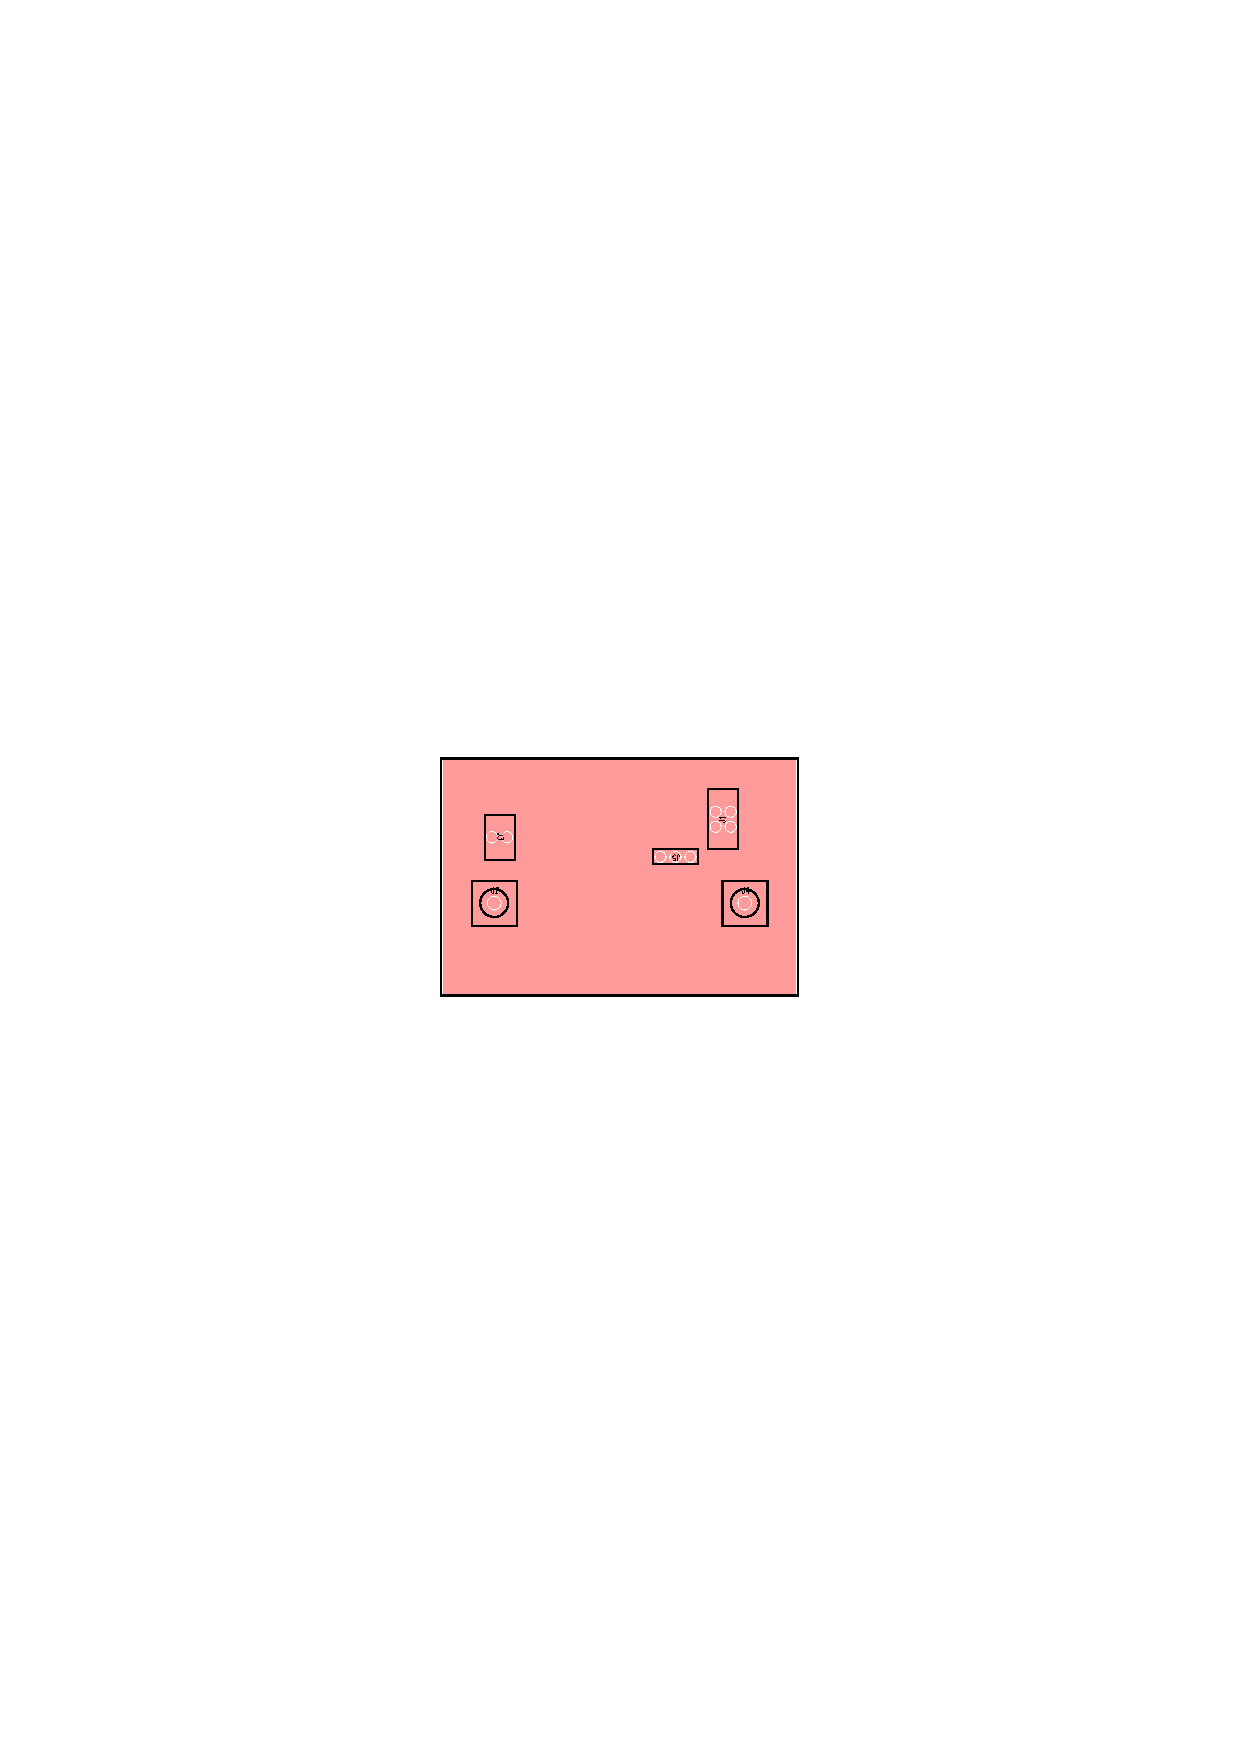
\includegraphics[trim = 7.3cm 12.7cm 7.3cm 12.7cm, clip, width=6.5cm]{../../CAM_DOC/O1.pdf}
  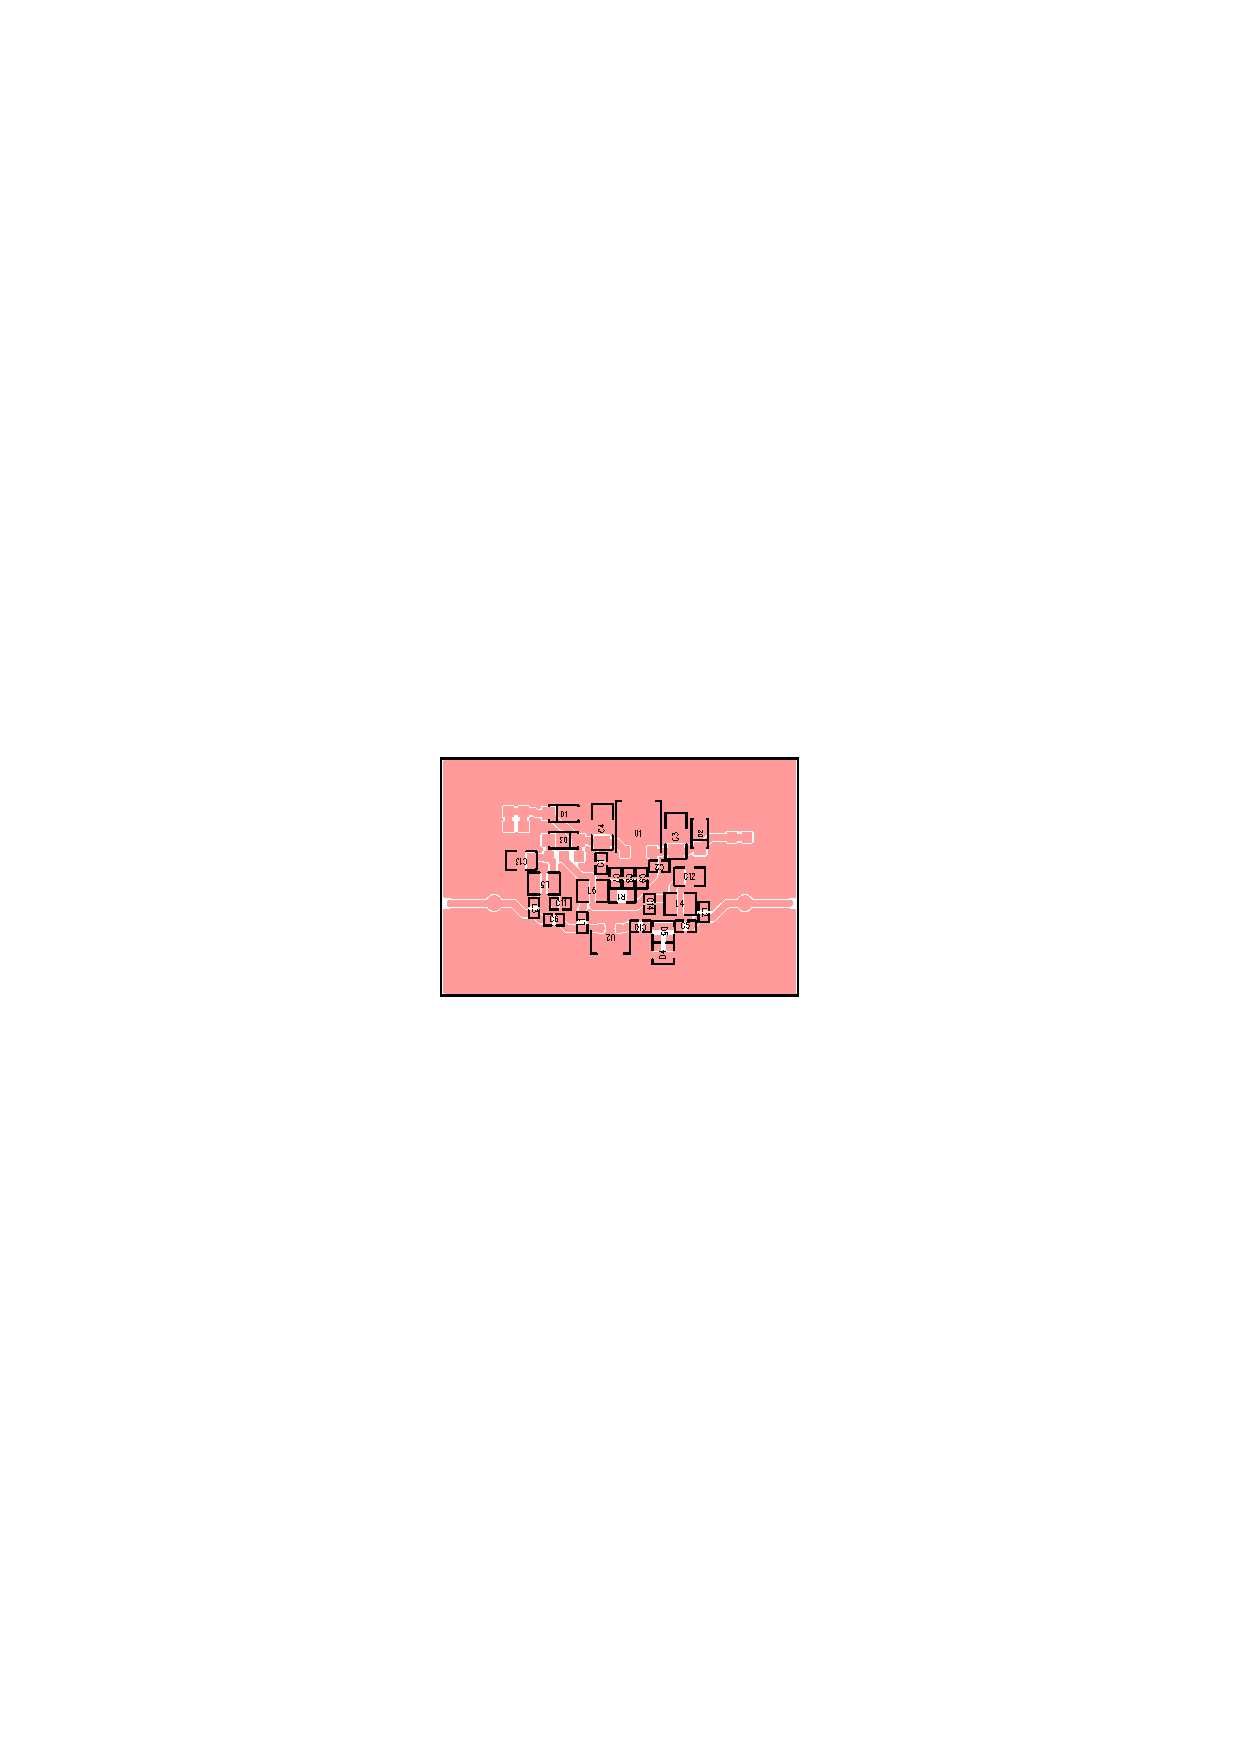
\includegraphics[trim = 7.3cm 12.7cm 7.3cm 12.7cm, clip, width=6.5cm]{../../CAM_DOC/O2.pdf}
  \caption{Osazovací plán horní a spodní strany plošného spoje}
  \label{fig:osazovaci_plan}
\end{figure}

\begin{savenotes}
\begin{table}[h!]
\begin{center}
\begin{tabular}{ |c|c|c|c| }
\hline 
Počet & Označení & Typ  & Pouzdro  \\ 
\hline 
7	&	C1,C2,C5,C6,C10,C11,C14	&	C0805	&	100nF	\\
2	&	C3,C4	&	ELYTC	&	47uF	\\
1	&	C7	&	C0805	&	68pF	\\
1	&	C8	&	C0805	&	1nF	\\
1	&	C9	&	C0805	&	1uF	\\
2	&	C12,C13	&	ELYTB	&	10uF/16V	\\
3	&	D1,D2,D3	&	SMA	&	M4	\\
2	&	D4,D5	&	SOT23	&	BAR43SSMD	\\
1	&	J1	&	JUMP2X4	&	JUMP2X4	\\
2	&	J2,J4	&	SMA6251A13G50	&	SMA6251A13G50	\\
1	&	J3	&	JUMP2X3	&	JUMP2X3	\\
1	&	J5	&	JUMP3	&	Power Bypass	\\
3	&	L1,L2,L3	&	R0805	&	BLM21PG300SN1D	\\
3	&	L4,L5,L6	&	L1812	&	CC453232-1R2KL	\\
1	&	R1	&	R1206	&	10R/0R	\\
1	&	U1	&	TO252	&	LM78M05CDT	\\
1	&	U2	&	SOT89	&	ADL5536	\\
\hline 
\end{tabular}
\end{center}
\caption{Seznam součástek pro všechny varianty osazení plošného spoje.}
\label{seznam_soucastek}
\end{table}
\end{savenotes}

\newpage

\subsubsection{Nastavení}
Nastavení modulu se provádí jumperem na jeho vrchní straně. 


\begin{thebibliography}{99}
\bibitem{Si570board}{Původní konstrukce Si570 Board } 
\href{http://wb6dhw.com/inactive.html}{http://wb6dhw.com/inactive.html}

\end{thebibliography}
\end{document}